\subsection{Simplified models spectra philosophy and naming convention}
\def\chitz{\ensuremath{\widetilde{\chi}^0_2}}
\def\chiz{\ensuremath{\widetilde{\chi}^0_1}}
\def\chipm{\ensuremath{\widetilde{\chi}^\pm_1}}
\def\chimp{\ensuremath{\widetilde{\chi}^\mp_1}}
\def\tchi{\ensuremath{\widetilde{\chi}}}
\def\gl{\tilde{g}}
\def\sTop{\ensuremath{\tilde{t}}\xspace}
\def\st{\ensuremath{\tilde{t}}\xspace}
\def\slep{\ensuremath{\tilde{l}}\xspace}
\def\snu{\ensuremath{\tilde{\nu}}\xspace}
\def\sBottom{\tilde{b}}
\def\sb{\tilde{b}}
\def\sq{\tilde{q}}
\def\sb{\tilde{b}}
\def\st{\tilde{t}}
\def\fb{\mathrm{fb}}
\def\to{\rightarrow}
\def\first{1$^\mathrm{st}$}
\def\second{2$^\mathrm{nd}$\xspace}
\def\third{3$^\mathrm{rd}$\xspace}
\def\spacer{\hspace*{10mm} }
\definecolor{red}{rgb}{.6,.02,.02} 
%\newcommand\fixme[1]{{\begin{color}{red}FIXME #1\end{color}}}
\newcommand\fixme[1]{{\color{red}FIXME #1}}
\newcommand\model[1]{{\tt #1}}
\newcommand\url[1]{{\nopagebreak{\tt #1}}}
\newcommand\smallurl[1]{{\small \tt #1}}
\newcommand{\AlphaT}{\ensuremath{\alpha_{\mathrm{T}}}\xspace} 
\newcommand{\ATLLepStop}{ATL lep-$\tilde{t}$}
\newcommand{\ATLHadStop}{ATL had-$\tilde{t}$}
\newcommand{\SSnoHT}{SSnoH$_{\mathrm{T}}$}
\newcommand{\HsTjets}{\ensuremath{\not\!\!\mathrm{H}_{\mathrm{T}}}+jets\xspace}
\newcommand{\MTtwo}{\ensuremath{{M}_{\mathrm{T2}}}\xspace}  
\newcommand{\emu}{\ensuremath{e/\mu}\xspace}
\newcommand{\ETslash}{\ensuremath{\not\!\!\rm{E}_{\mathrm{T}}}\xspace} 
\newcommand{\ZMET}{Z+\ETslash}
\newcommand{\sigmaXBF}{\mbox{\ensuremath{\sigma\times\mathcal{B}}}\xspace}

\label{ssec:names}

The guiding principle behind the SMS decomposition is the assumption that most experimental searches
for new physics are insensitive to various specific details of the BSM model, such as the spin, charge and interactions
of the new physical states, {\it as long as they give rise to the same signal topology}. 
This assumption is clearly violated by searches which strongly rely on specific details of the
signal, such as spin correlations and properties of off-shell states. Nonetheless, 
most current experimental analyses aim for model independent constraints and can 
be interpreted within the SMS framework.
In these cases, to a first approximation, it is possible to reduce all the properties of a BSM model to its mass
spectrum, branching ratios (BRs) and production cross-sections\footnote{Clearly the calculation of branching ratios and production cross-sections depend on the specific properties of the new physical states and their interactions.
 Nonetheless, in the SMS approach all the complexity of the BSM model can be replaced
by the knowledge of its BRs, cross-sections and mass spectrum.}.
With this knowledge we can decompose the BSM signal in a series of independent signal topologies with their specific weights given
by the corresponding production cross-section times branching ratio (\sigmaXBF). Such decomposition is extremely helpful to cast the theoretical
predictions of a specific BSM model in a model-independent framework, which can then be compared against model-independent experimental searches.
The specific details of the decomposition procedure will be discussed in Sec.\ref{ssec:decomp}.


In order to clarify the above statements and set some of the notation used here, we show in Fig.\ref{fig:SMSexample} two common topologies which appear
in R-parity conserving supersymmetric models. Although the diagrams in Fig.\ref{fig:C1N2} and \ref{fig:SLSN} have a very distinct particle (and spin) content, 
most experimental searches sensitive to the "naked" diagram (SMS topology) of Fig.\ref{fig:C1N2naked} can be used to constrain the other two.

\begin{figure}[h!t]
\begin{center}
\begin{tabular}{lcr}
\subfigure[\label{fig:C1N2}$\tchi_1^+$,$\chitz$ topology]{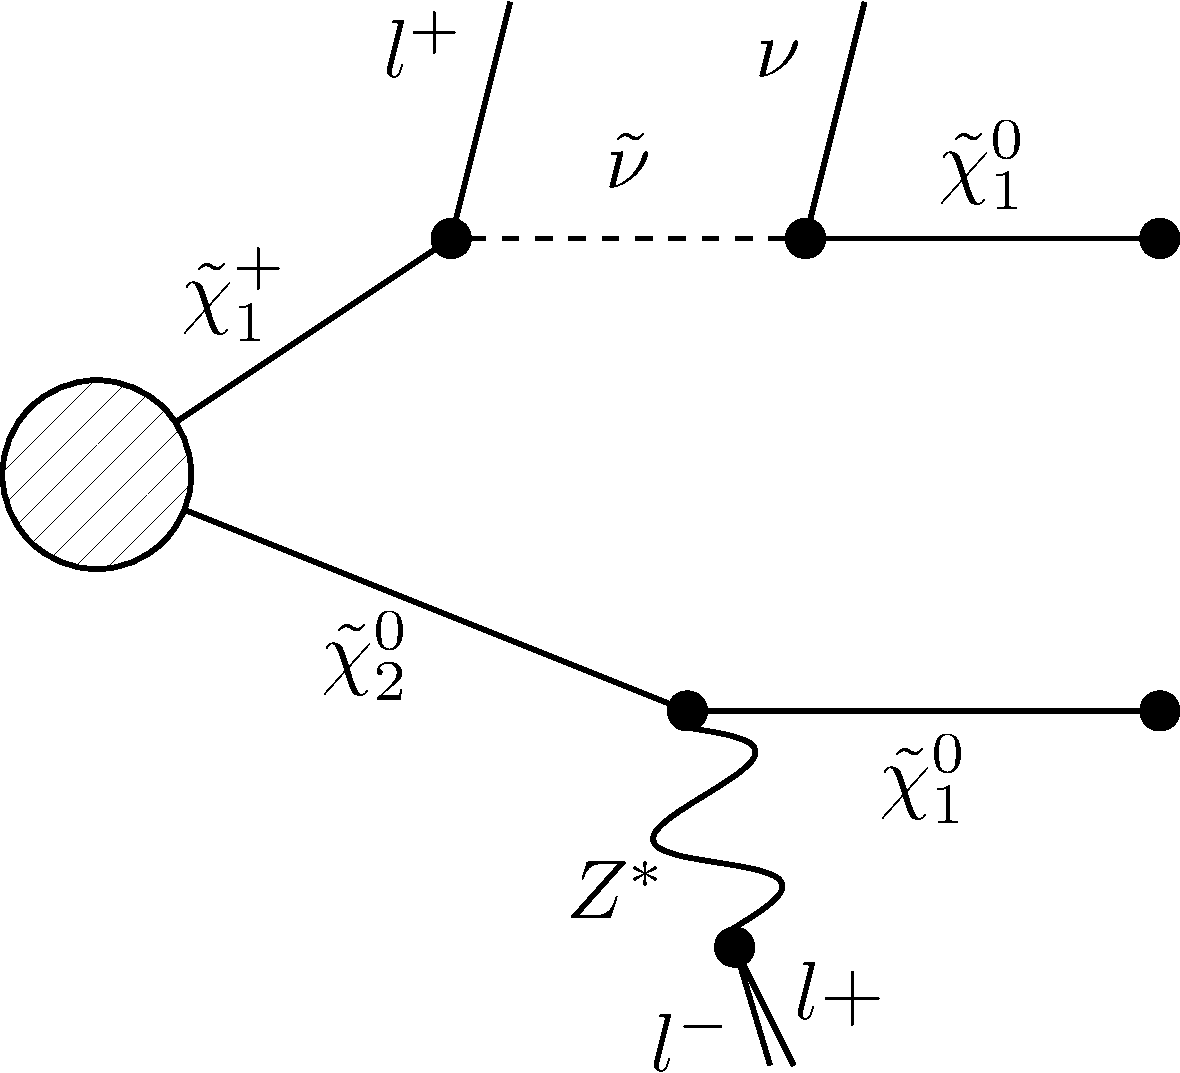
\includegraphics[width=0.25\linewidth]{figures/C1N2.pdf}}\spacer &
\subfigure[\label{fig:SLSN}$\slep_1^+$,$\snu$ topology]{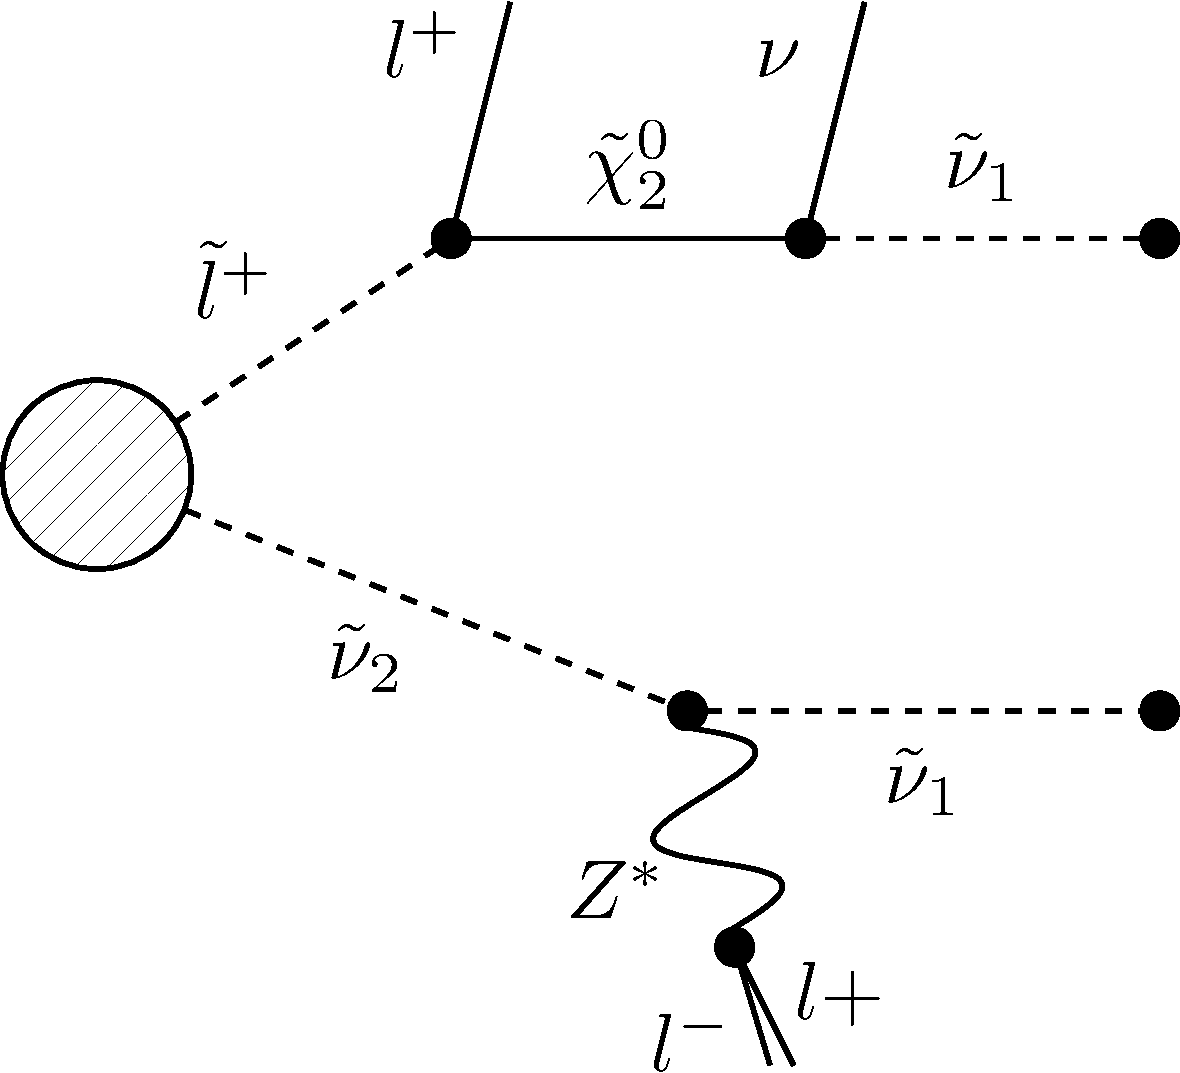
\includegraphics[width=0.25\linewidth]{figures/SLSN.pdf}}\spacer &
\subfigure[\label{fig:C1N2naked}SMS equivalent topology]{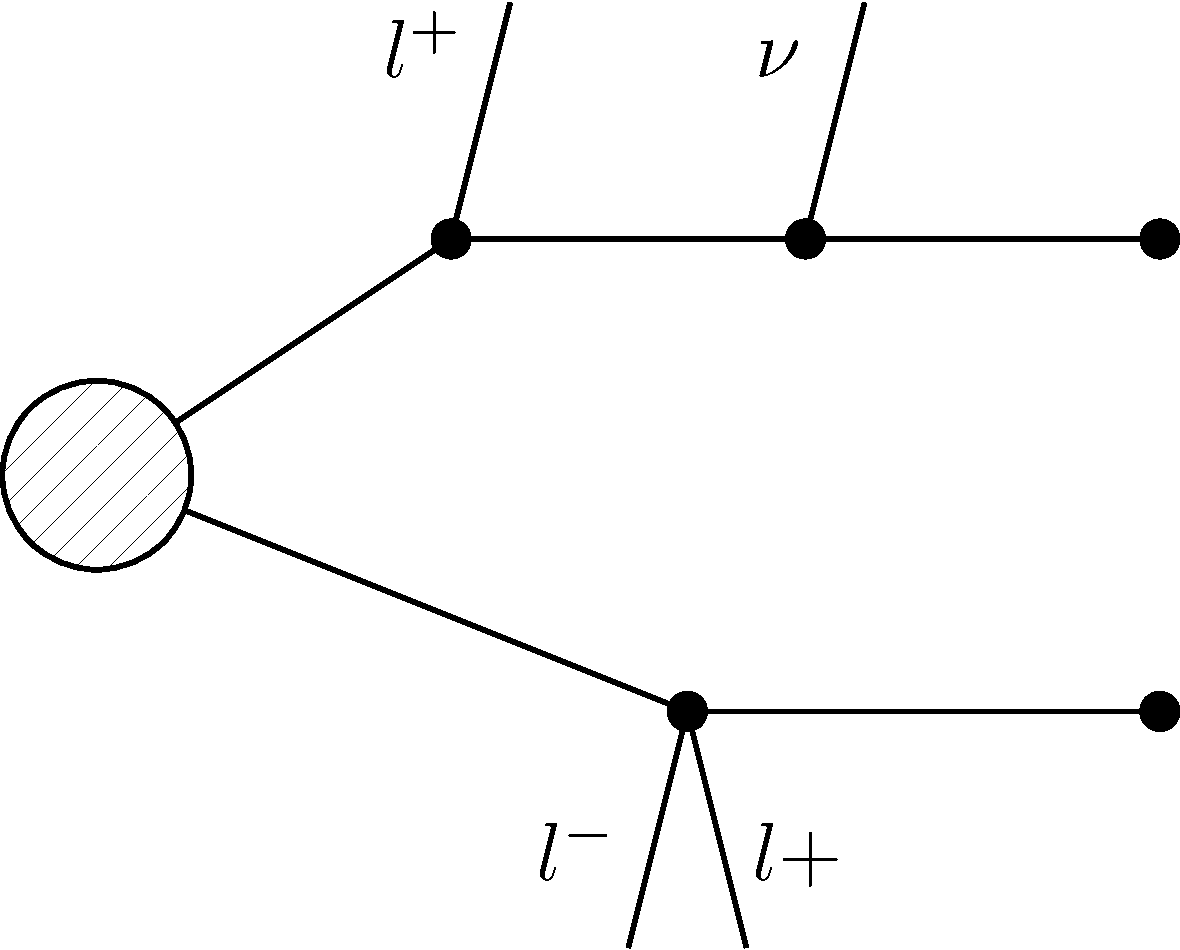
\includegraphics[width=0.27\linewidth]{figures/C1N2naked.pdf}}\spacer \\
\end{tabular}
\caption{Some examples of model-dependent signal topologies and their SMS equivalent.}
\label{fig:SMSexample}
\end{center}
\end{figure}

Since here we only consider models with a $\mathbb{Z}_2$ symmetry (such as R-Parity, T-Parity or KK-Parity),
the possible signal topologies will always consist of 
pair production of new ($\mathbb{Z}_2$-odd) particle states\footnote{Throughout this work we 
ignore BSM particles which are $\mathbb{Z}_2$-even, such as heavy higgses in the MSSM. These
cases will be discussed in future work.},
which decay as $P \to P' + $SM particles,
where $P$ and $P'$ are the parent and daughter BSM particles, respectively.
Hence all topologies will be of the form shown in Fig.\ref{fig:GenSMSTop}, consisting of two branches, each one characterized by its number of vertices and the SM particles appearing in each vertex. 
In our notation all particles appearing in the SMS topology
 (both $\mathbb{Z}_2$-even and $\mathbb{Z}_2$-odd) are on-shell. 
The case of off-shell decays are always included as 3-body decays, with no mention to off-shell states.
Therefore all the relevant information (in the SMS framework) of such a diagram can be 
reduced to three main objects:
\begin{itemize}
\item The diagram topology (number of vertices and SM final state particles in each vertex)
\item The masses of the BSM particles ($\mathbb{Z}$-odd) appearing in the diagram
\item The diagram weight (\sigmaXBF).
\end{itemize}

In order to classify the possible signal topologies we choose to label them according to the
SM states appearing in each vertex, as well as the number of vertices in each branch\footnote{Although the experimental collaborations have already introduced their
own naming convention, we choose not to use them, since they are more strongly biased by specific
BSM models.}.
To illustrate our notation, we show in Fig.\ref{fig:SMSlabel} the labeling scheme used to describe the 
diagram in Fig.\ref{fig:C1N2naked}.
Each outer pair of brackets refer to a branch ($[B_1,B_2]$). 
Inside each branch bracket, the inner brackets
correspond to the lists of SM particles coming out of each vertex.
Note that there is no mention to the intermediate BSM particles ($\tchi_1$, $\slep$,...),
what makes our method explicitly model independent. The only information kept from the BSM states
are their masses. For the SMS topology of Fig.\ref{fig:C1N2naked}, we have $[B_1,B_2]$, with $B_1 = [[l^+],[\nu]]$ and $B_2 = [[l^+,l^-]]$, 
as illustrated in Fig.\ref{fig:SMSlabel}. With the labeling scheme just introduced it becomes obvious
that the two (model dependent) diagrams in Figs.\ref{fig:C1N2} and \ref{fig:SLSN} have identical SMS topologies.

\begin{figure}[h!t]
\begin{center}
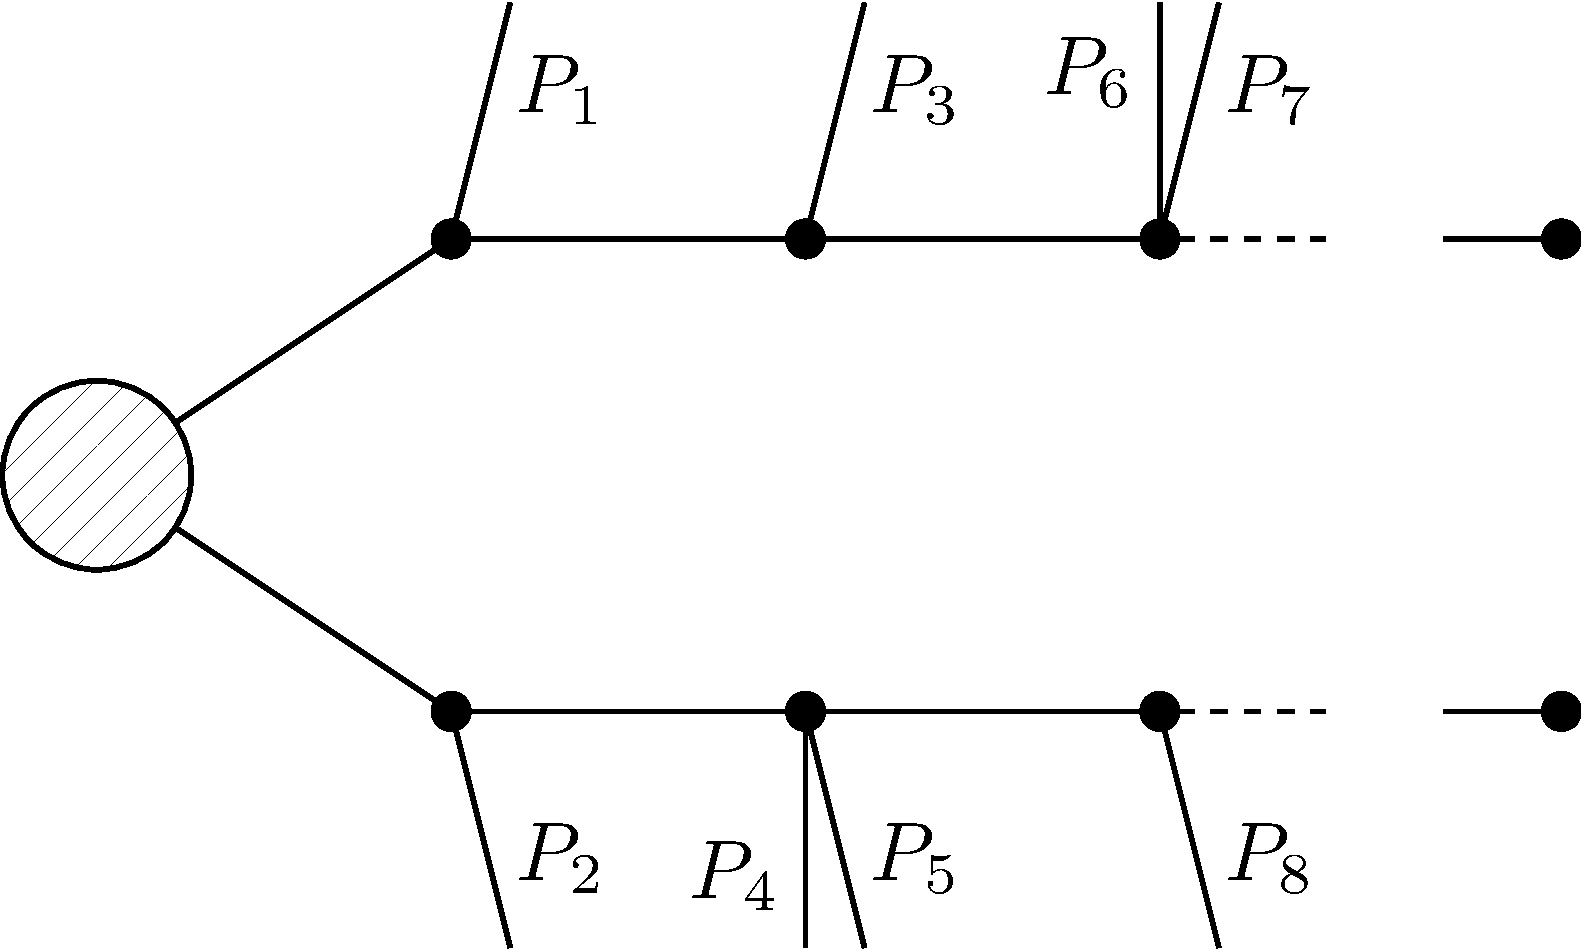
\includegraphics[width=0.35\linewidth]{figures/GeneralTop.pdf}
\caption{The general type of SMS topology considered in this document. $P_i$ label the SM final state particles.}
\label{fig:GenSMSTop}
\end{center}
\end{figure}


\begin{figure}[h!t]
\begin{center}
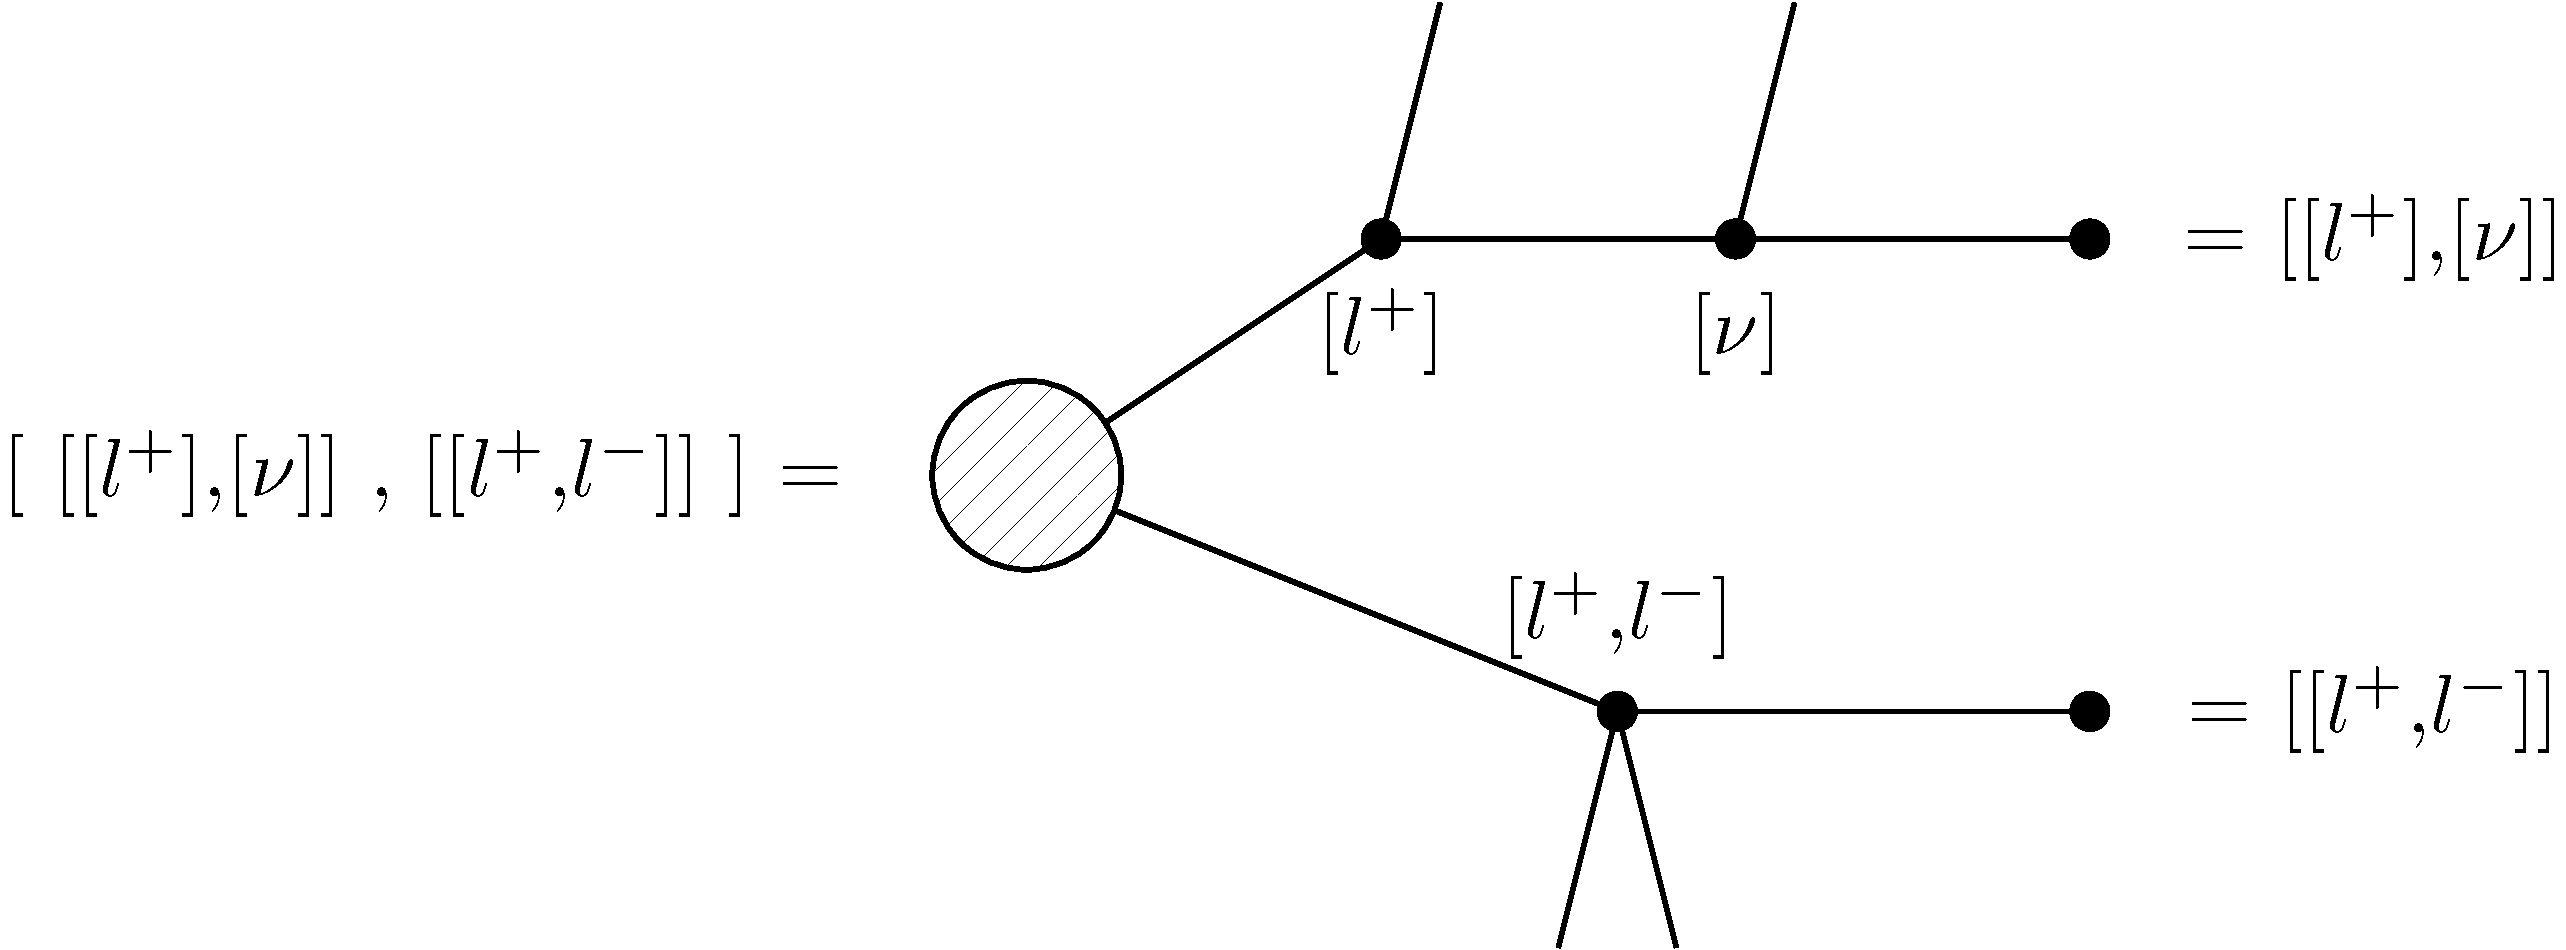
\includegraphics[width=0.7\linewidth]{figures/C1N2labels.pdf}
\caption{The labeling scheme adopted here applied to the diagram in Fig.\ref{fig:C1N2naked}.}
\label{fig:SMSlabel}
\end{center}
\end{figure}



\subsection{Anatomy of an SMS result}
\label{ssec:smsstatistics}


When interpreting the experimental results in the SMS framework, the
BSM model is completely fixed by its SMS topologies 
(defined by the number of vertices and the SM particles appearing in each vertex), 
the masses appearing in the topologies and the topology cross-sections.
In most cases the experimental collaborations choose a single SMS topology
(some exceptions are discussed below) and scan over the unknown masses or a subset of the masses
(with simplifying assumptions for the other masses).
Then the only unkown is the topology cross-section, which can be constrained using data.
The CMS and ATLAS collaborations typically use such scans to produce two types
of resulting plots: given a well-defined signal region, the collaborations
can report the analysis' acceptance times efficiency values ($A \times
\epsilon$), as a function of the mass parameters for an assumed SMS topology. 
Such a result is shown in Fig.~\ref{fig:smsexampleeff}. 
In the second case, a 95\% confidence level upper limit (UL) on
the SMS topology's cross section ($\sigma$) is computed, as a function
of the topology's mass parameters. A typical result can be seen in
Fig.~\ref{fig:smsexampleul}: the colors show the binned values for the upper limit on $\sigma$.
Finally, assuming theoretical ``reference'' cross sections for each mass value,
an exclusion curve is produced. Therefore, the exclusion curves can only be
applied to models with the same reference cross-section assumed by the collaboration.
Also, as the experimental searches become more complex and deviate from the simple cut and count analyses,
efficiency plots can no longer be produced \fixme{true?}. Hence this document builds upon the 
95\% upper limits on $\sigma$ -- neither the
efficiency plots nor the exclusion lines are of any relevance for this work.

\begin{figure}[ht!]
\begin{center}
\begin{tabular}{lr}
\subfigure[\label{fig:smsexampleeff}efficiency plot]{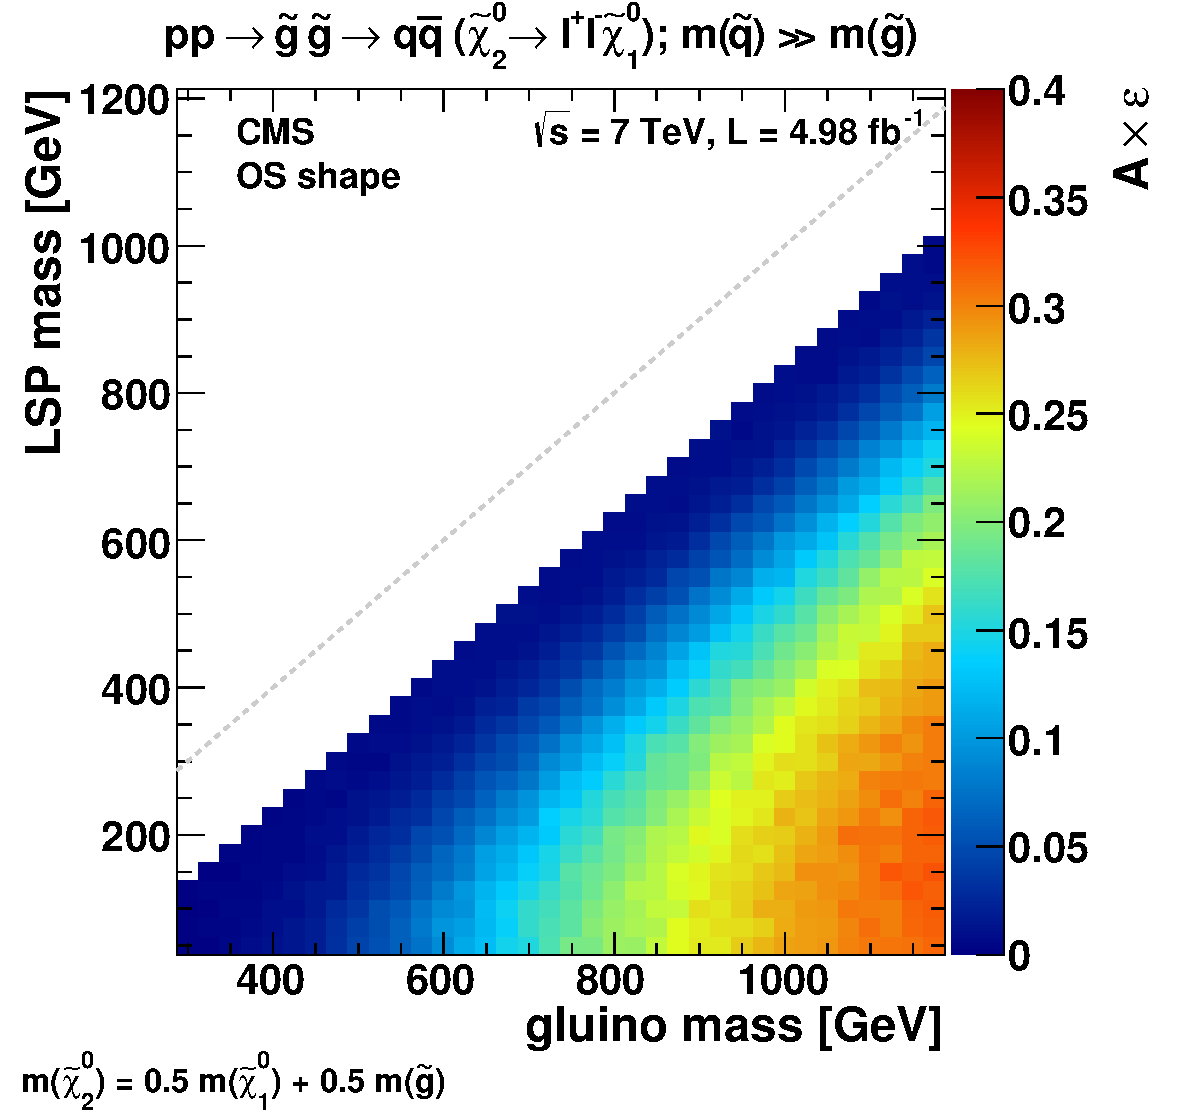
\includegraphics[width=0.5\linewidth]{figures/h_eff_T3lh_OSshape.pdf}} &
\subfigure[\label{fig:smsexampleul}upper limits on production cross
section]
{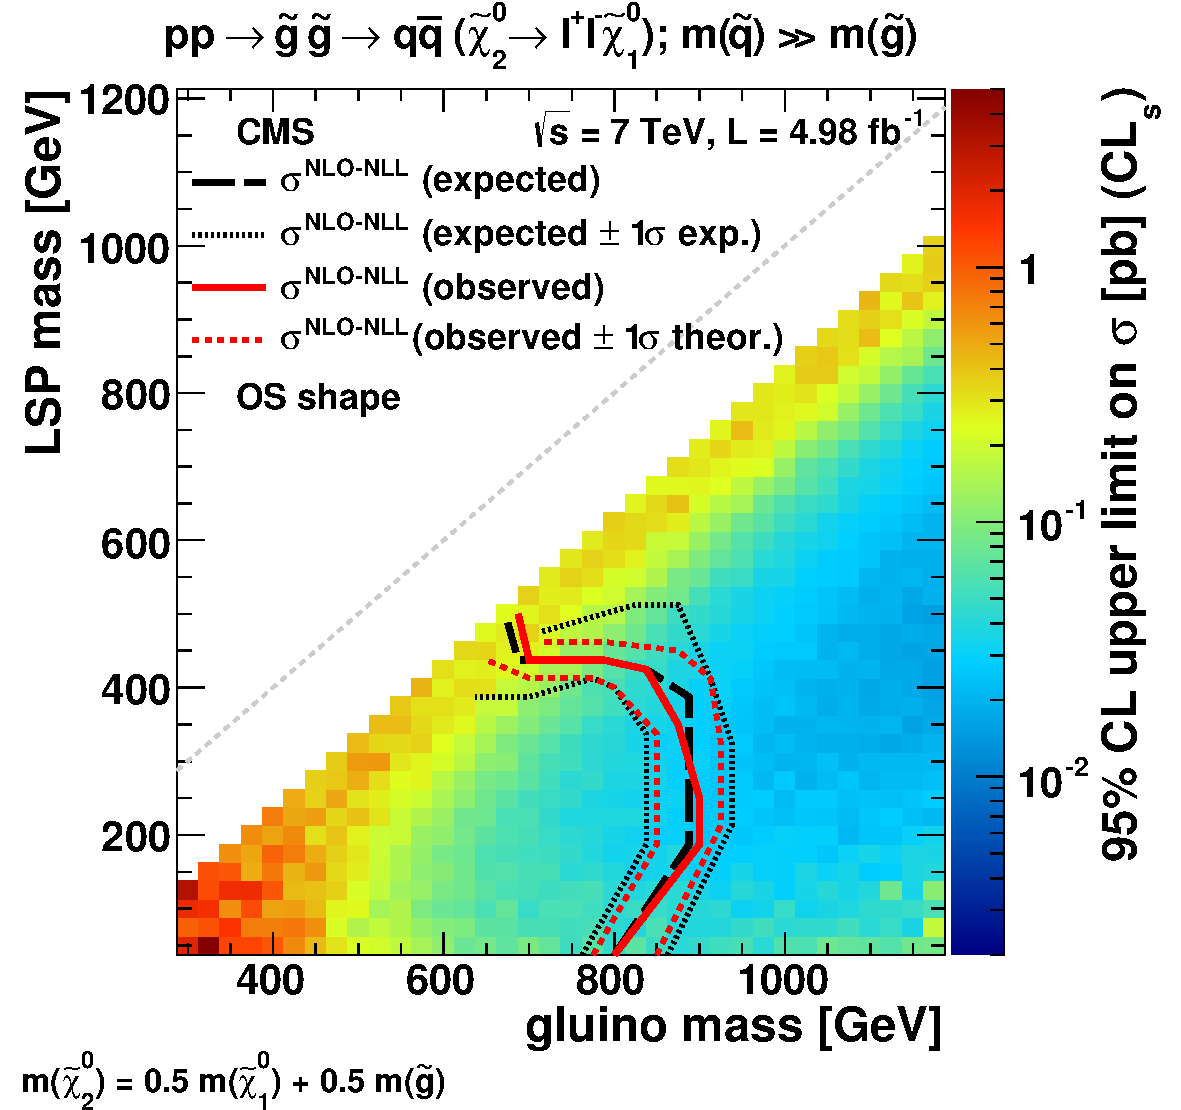
\includegraphics[width=0.5\linewidth]{figures/h_limit_T3lh_OSshape.pdf}}
\\
\end{tabular}
\caption{An example of an SMS result of the CMS collaboration, taken
from~\cite{cms:2013wc}.}
\label{fig:smsexample}
\end{center}
\end{figure}

In some particular cases, motivated by specific BSM models, the experimental collaborations
choose to apply the experimental constraints to a certain combination of SMS topologies.
The simplest example is the CMS dilepton search\cite{SUS-12-022} 
for slepton pair production and decay: $\slep^+ + \slep^- \to (l^+ \chiz) + (l^- \chiz)$,
where $\slep = \tilde{e}, \tilde{\mu}$.
Under the assumption that the selectron and smuon are degenerate, the experimental collaboration
do not constraint each flavor individually, but choose to constraint the sum of the two SMS topology
 cross-sections instead: $\sigma([[[e^+]],[[e^-]]]) + \sigma([[[\mu^+]],[[\mu^-]]])$,
where we are using the notation introduced in Sec.\ref{ssec:names}. In such cases, the experimental
constraints can only be applied under some assumptions. For the slepton case just
mentioned the assumption is that each single topology ($[[[e^+]],[[e^-]]]$ or $[[[\mu^+]],[[\mu^-]]]$)
contributes equally to the sum ($\sigma([[[e^+]],[[e^-]]]) = \sigma([[[\mu^+]],[[\mu^-]]])$). 
This condition can be relaxed if we assume that the signal efficiency for the SMS topology
with muons in the final state is higher than for electrons, so it is enough to require 
$\sigma([[[e^+]],[[e^-]]]) \leq \sigma([[[\mu^+]],[[\mu^-]]])$. 
Other examples of experimental constraints on sums of topologies can be seen in Table~\ref{tab:LHCresults}
and envolve the SMS topologies appearing in the production of electroweak inos 
decaying through sleptons and/or sneutrinos\cite{SUS-12-022,ATLAS-CONF-2013-035,ATLAS-CONF-2013-028,ATLAS-CONF-2013-036}.



Finally, we point out that it is a long-standing wish of the authors that the experimental
collaborations publish not only the 95\% upper limits, but rather the entire
likelihoods.  This would e.g. allow combinations of LHC results with
uncorrelated non-LHC measurements.  
A combination of several LHC results would still not be feasible because 
the correlations between the SMS results are unknown.
It is an even longer term vision that all ingredients that enter
into the statistical procedure are published also;
in an ideal world a user of the LHC results would be able to produce 
a likelihood for any combination of SMS results published, be they from CMS or
ATLAS.

\subsection{LHC results used}
\label{ssec:lhc}

In our subsequent results we consider the latest ATLAS and CMS analyses (with results
interpreted in terms of simplified models) for R-Parity conserving supersymmetric models. The complete list of
results used are shown in Table \ref{tab:LHCresults} in the Appendix, where we also show
the SMS topologies constrained by each analysis.
As discussed in Sec.\ref{ssec:smsstatistics}, some of the results constrain
sums of single SMS topologies and include additional assumptions about
the contribution of each topology. Whenever such results are applied to exclude a model 
we verify that the respective assumptions are satisfied.


